\problemname{Fair and Square}

\newcommand*{\name}{Felix}

\name{} has ordered a large rectangular pizza for his birthday party.
He only quickly went to the kitchen to grab some plates and cutlery, and when he came back his guests had already started helping themselves to various parts of the pizza.
The pizza, which originally was made up of $h\times w$ square pieces of equal size, is now missing some of these pieces:

\begin{figure}[!h]
  \centering
  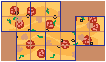
\includegraphics[width=0.62\textwidth]{pizza.pdf}
  \caption{Illustration of the first sample case, with a division into squares of side length $2$.}
\end{figure}

To ensure that the distribution of the rest of the pizza proceeds in a much more orderly fashion, \name{} wants to divide up the remaining pizza into larger square shaped areas.
\name{} can only cut along the grid lines and cannot rearrange any parts of the pizza.
Each square should have the same side length, which should be as large as possible in order to minimize the number of plates needed.

Find this largest possible side length.
Note that an answer always exists because the pizza can always be divided into $1\times 1$ squares.

\vspace{-4mm}
\begin{Input}
  The input consists of:
  \begin{itemize}
    \item One line with two integers $h$ and $w$ ($1 \le h,w \le 2500$), the height and width of the grid.
    \item $h$ lines, each with a string of length $w$ consisting of `\texttt{\#}' (denoting pizza pieces that are still there) and `\texttt{.}' (denoting pizza pieces that have already been taken).
  \end{itemize}
  It is guaranteed that the input contains at least one `\texttt{\#}'.
\end{Input}

\vspace{-3mm}
\begin{Output}
  Output an integer, the largest possible side length such that the remaining pizza can be divided into squares of that side length.
\end{Output}
